\section{实验结果与分析}

本节汇总SM4-CBC算法在WSL-Arch(x86\_64)与QEMU-RISC-V(rv64)两个平台上的性能测试结果，
涵盖未优化版本（original）、查表优化版本（table）、多缓冲区并行加密（multi-buffer）以及
并行解密（decrypt parallel）共六种实现变体，覆盖O0、O1、O2、O3四个编译器优化级别
以及1/2/4/8线程配置。WSL-Arch平台每组测试数据规模为1MiB并重复100轮,QEMU-RISC-V平台每组测试数据规模为1MiB并重复20轮。两平台循环次数不同,因此本文主要比较吞吐量和相对趋势,不直接比较单次总运行时间。

\subsection{整体性能汇总}

表~\ref{tab:summary_throughput_t1}列出了单线程条件下各变体在O0与O3优化级别下的吞吐量数据，
反映算法本身优化（查表法）与编译器优化对基础性能的贡献。

\begin{table}[H]
\centering
\caption{单线程吞吐量汇总（MB/s）}
\label{tab:summary_throughput_t1}
\begin{tabular}{llrr}
\hline
\textbf{平台} & \textbf{变体} & \textbf{O0} & \textbf{O3} \\
\hline
\multirow{6}{*}{WSL-Arch (x86\_64)} 
    & single\_original     & 64.60 & 120.76 \\
    & single\_table        & 101.08 & 180.83 \\
    & multibuffer\_original & 64.86 & 120.88 \\
    & multibuffer\_table   & 101.33 & 180.86 \\
    & decrypt\_parallel\_original & 57.73 & 120.57 \\
    & decrypt\_parallel\_table   & 89.91 & 182.07 \\
\hline
\multirow{6}{*}{QEMU RISC-V (rv64)} 
    & single\_original     & 4.65  & 33.77 \\
    & single\_table        & 12.31 & 41.79 \\
    & multibuffer\_original & 4.38 & 42.24 \\
    & multibuffer\_table   & 12.07 & 48.47 \\
    & decrypt\_parallel\_original & 4.63 & 36.01 \\
    & decrypt\_parallel\_table   & 10.60 & 42.75 \\
\hline
\end{tabular}
\end{table}

注：本表数据来源于\verb|data/wsl_arch.csv|与\verb|data/sm4_qemu_results.csv|,均取单线程配置。multi-buffer在1线程下退化为单条独立CBC数据流,因此可与single版本对照验证实现开销。

\subsection{跨平台性能对比}

图~\ref{fig:platform_bar}展示了WSL-Arch与QEMU-RISC-V两个平台在不同优化级别下的整体吞吐量对比。
该图汇总了所有变体与线程配置的平均吞吐量，直观反映两个平台的绝对性能差距。由于WSL平台多线程能够映射到真实CPU核心,而QEMU中的RISC-V程序仍需经过模拟执行,两者的绝对吞吐量存在显著差异。

\begin{figure}[H]
    \centering
    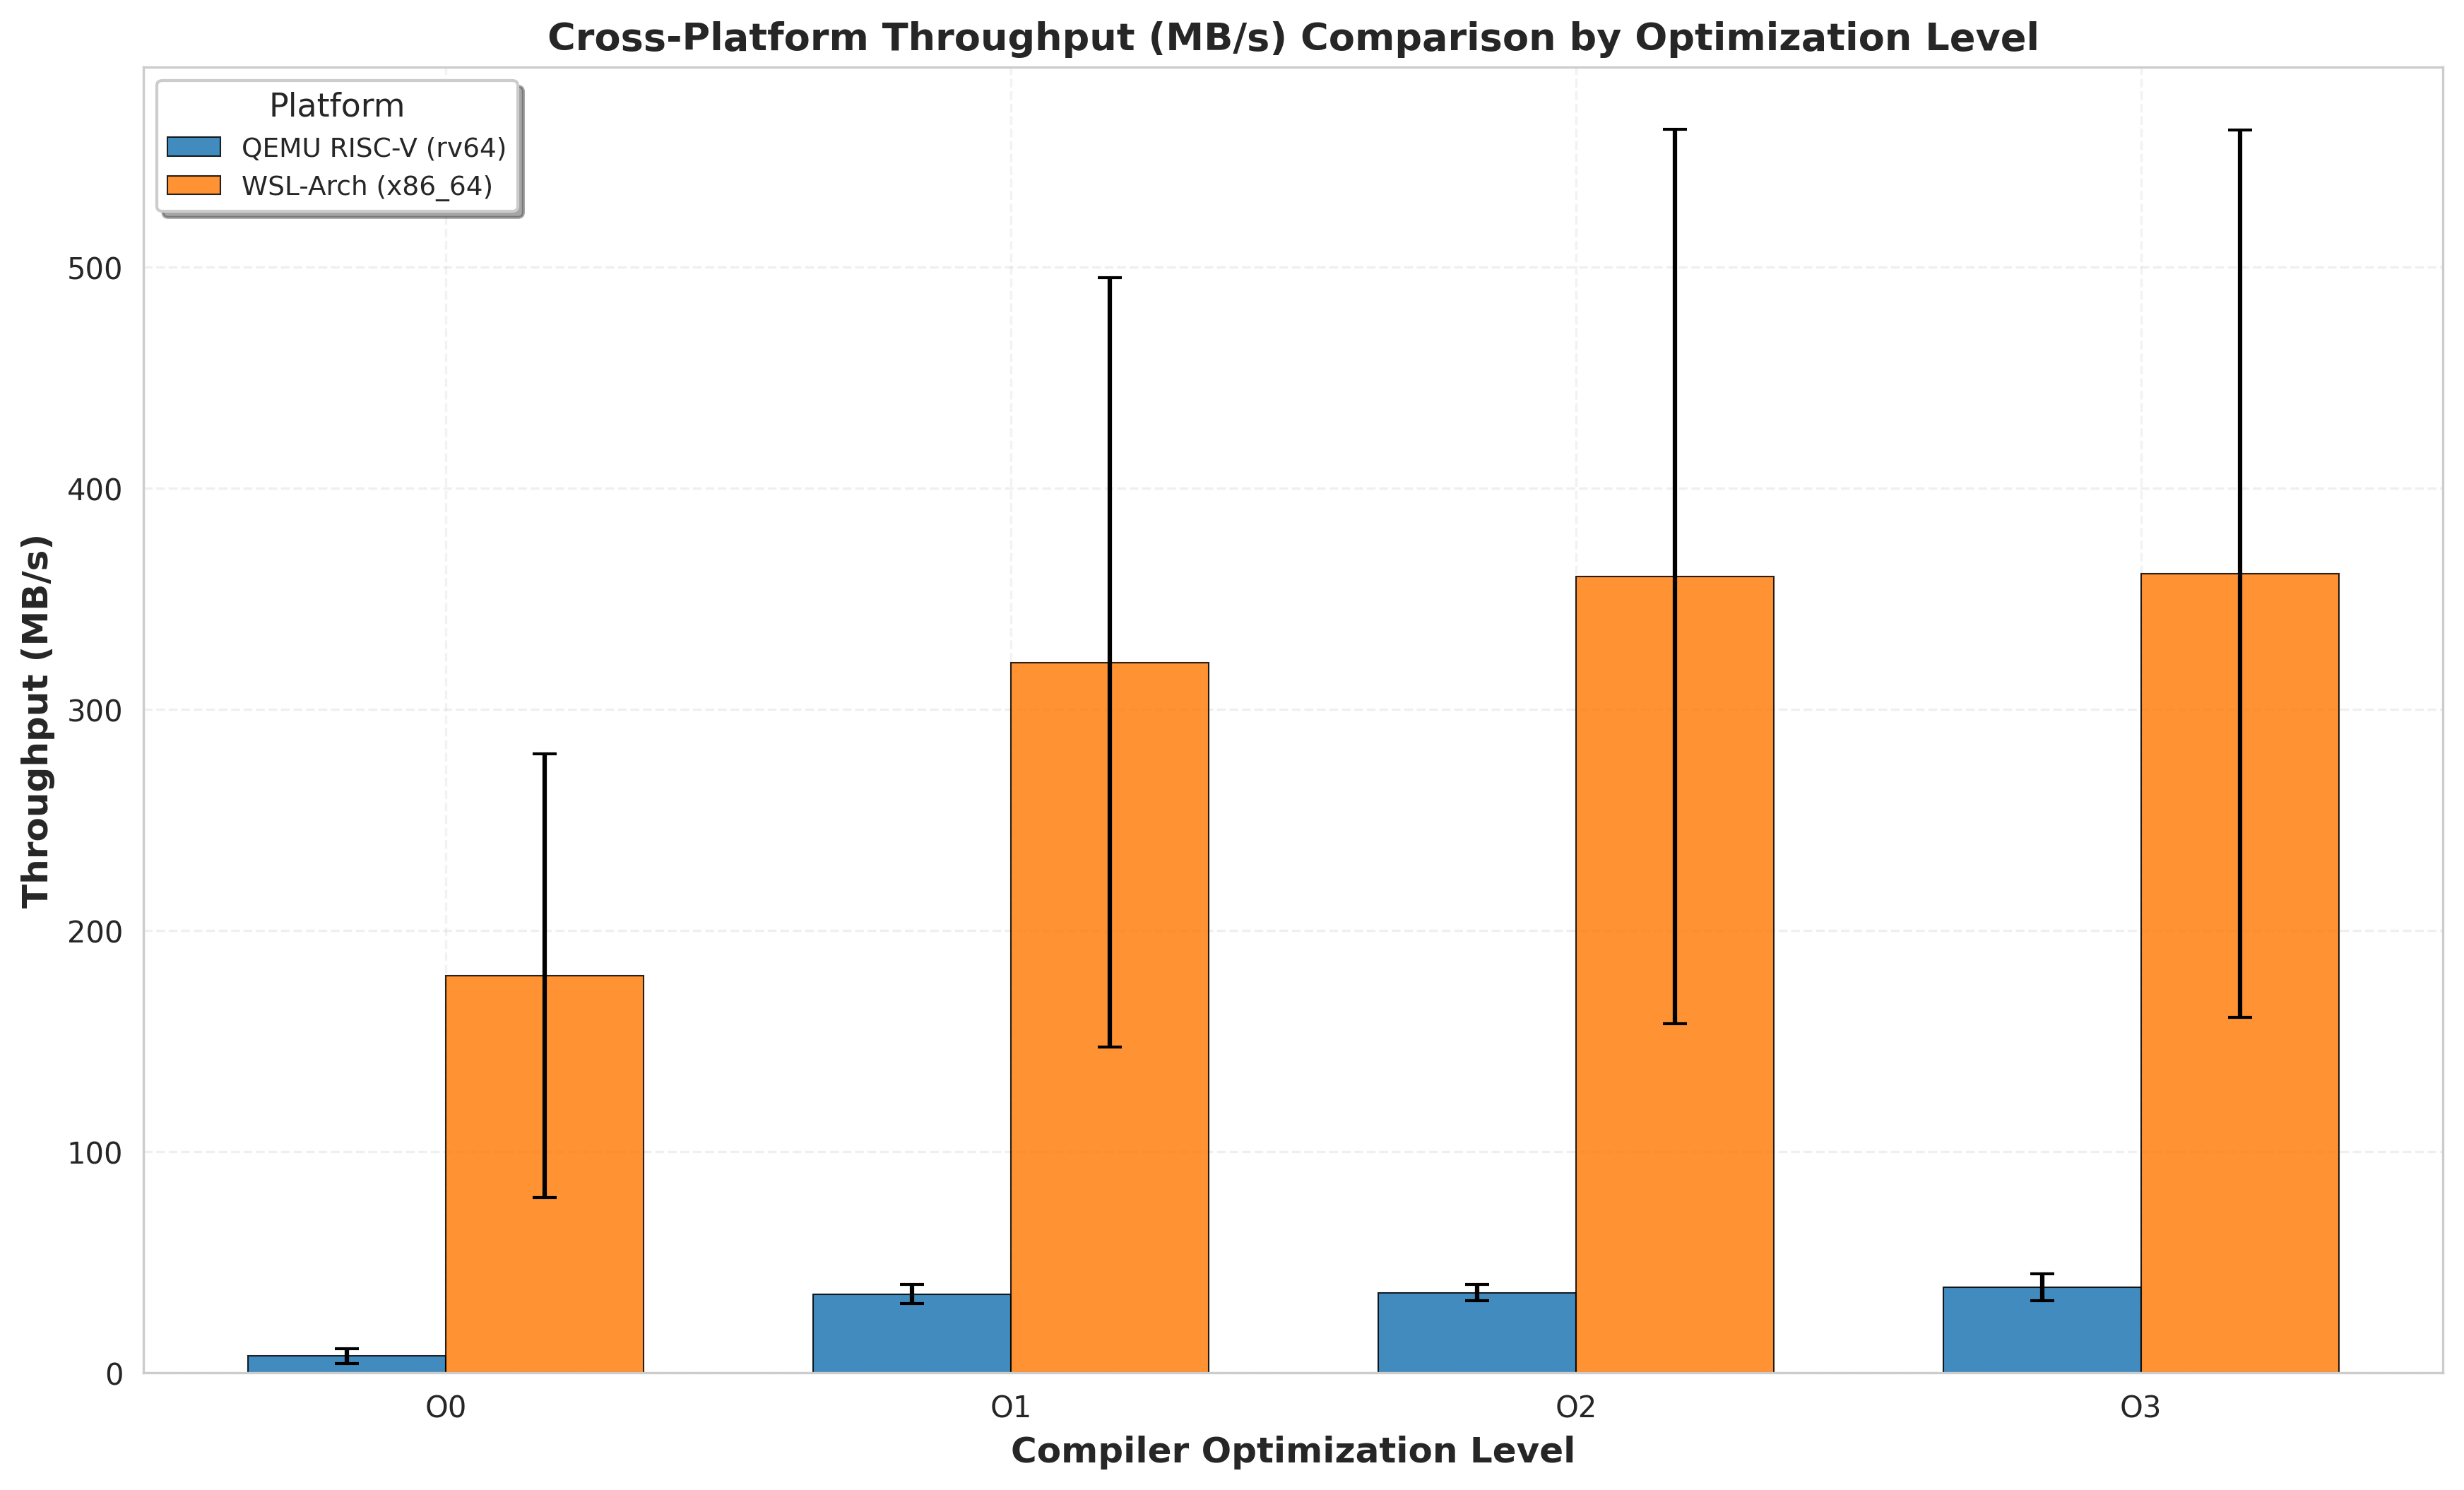
\includegraphics[width=\textwidth]{figure/bar_platform_throughput_MBps_by_opt.png}
    \caption{跨平台吞吐量对比（按优化级别分组）}
    \label{fig:platform_bar}
\end{figure}

从图中可以看出：
\begin{enumerate}
    \item WSL-Arch(x86\_64)平台在所有优化级别下吞吐量均显著高于QEMU-RISC-V仿真平台，
          这与x86\_64原生执行效率高于QEMU指令翻译仿真的预期一致。
    \item 编译器优化级别（O0→O3）对两个平台的性能提升趋势不同：
          WSL-Arch在O1即可获得主要收益，O2/O3继续小幅提升；
          QEMU-RISC-V从O0到O1提升最明显,O2/O3进一步改善但幅度较小。
    \item 单线程原始版本在QEMU-RISC-V上出现O1/O2略高于O3的情况,说明更高优化级别并不必然带来单个变体的最佳结果；但从所有变体的平均值看,O3仍取得最高整体吞吐量。
\end{enumerate}

\subsection{优化方法对比}

图~\ref{fig:method_wsl}与图~\ref{fig:method_qemu}分别展示了WSL-Arch与QEMU-RISC-V
在O3优化级别下，六种变体在不同线程数下的吞吐量对比。

\begin{figure}[H]
    \centering
    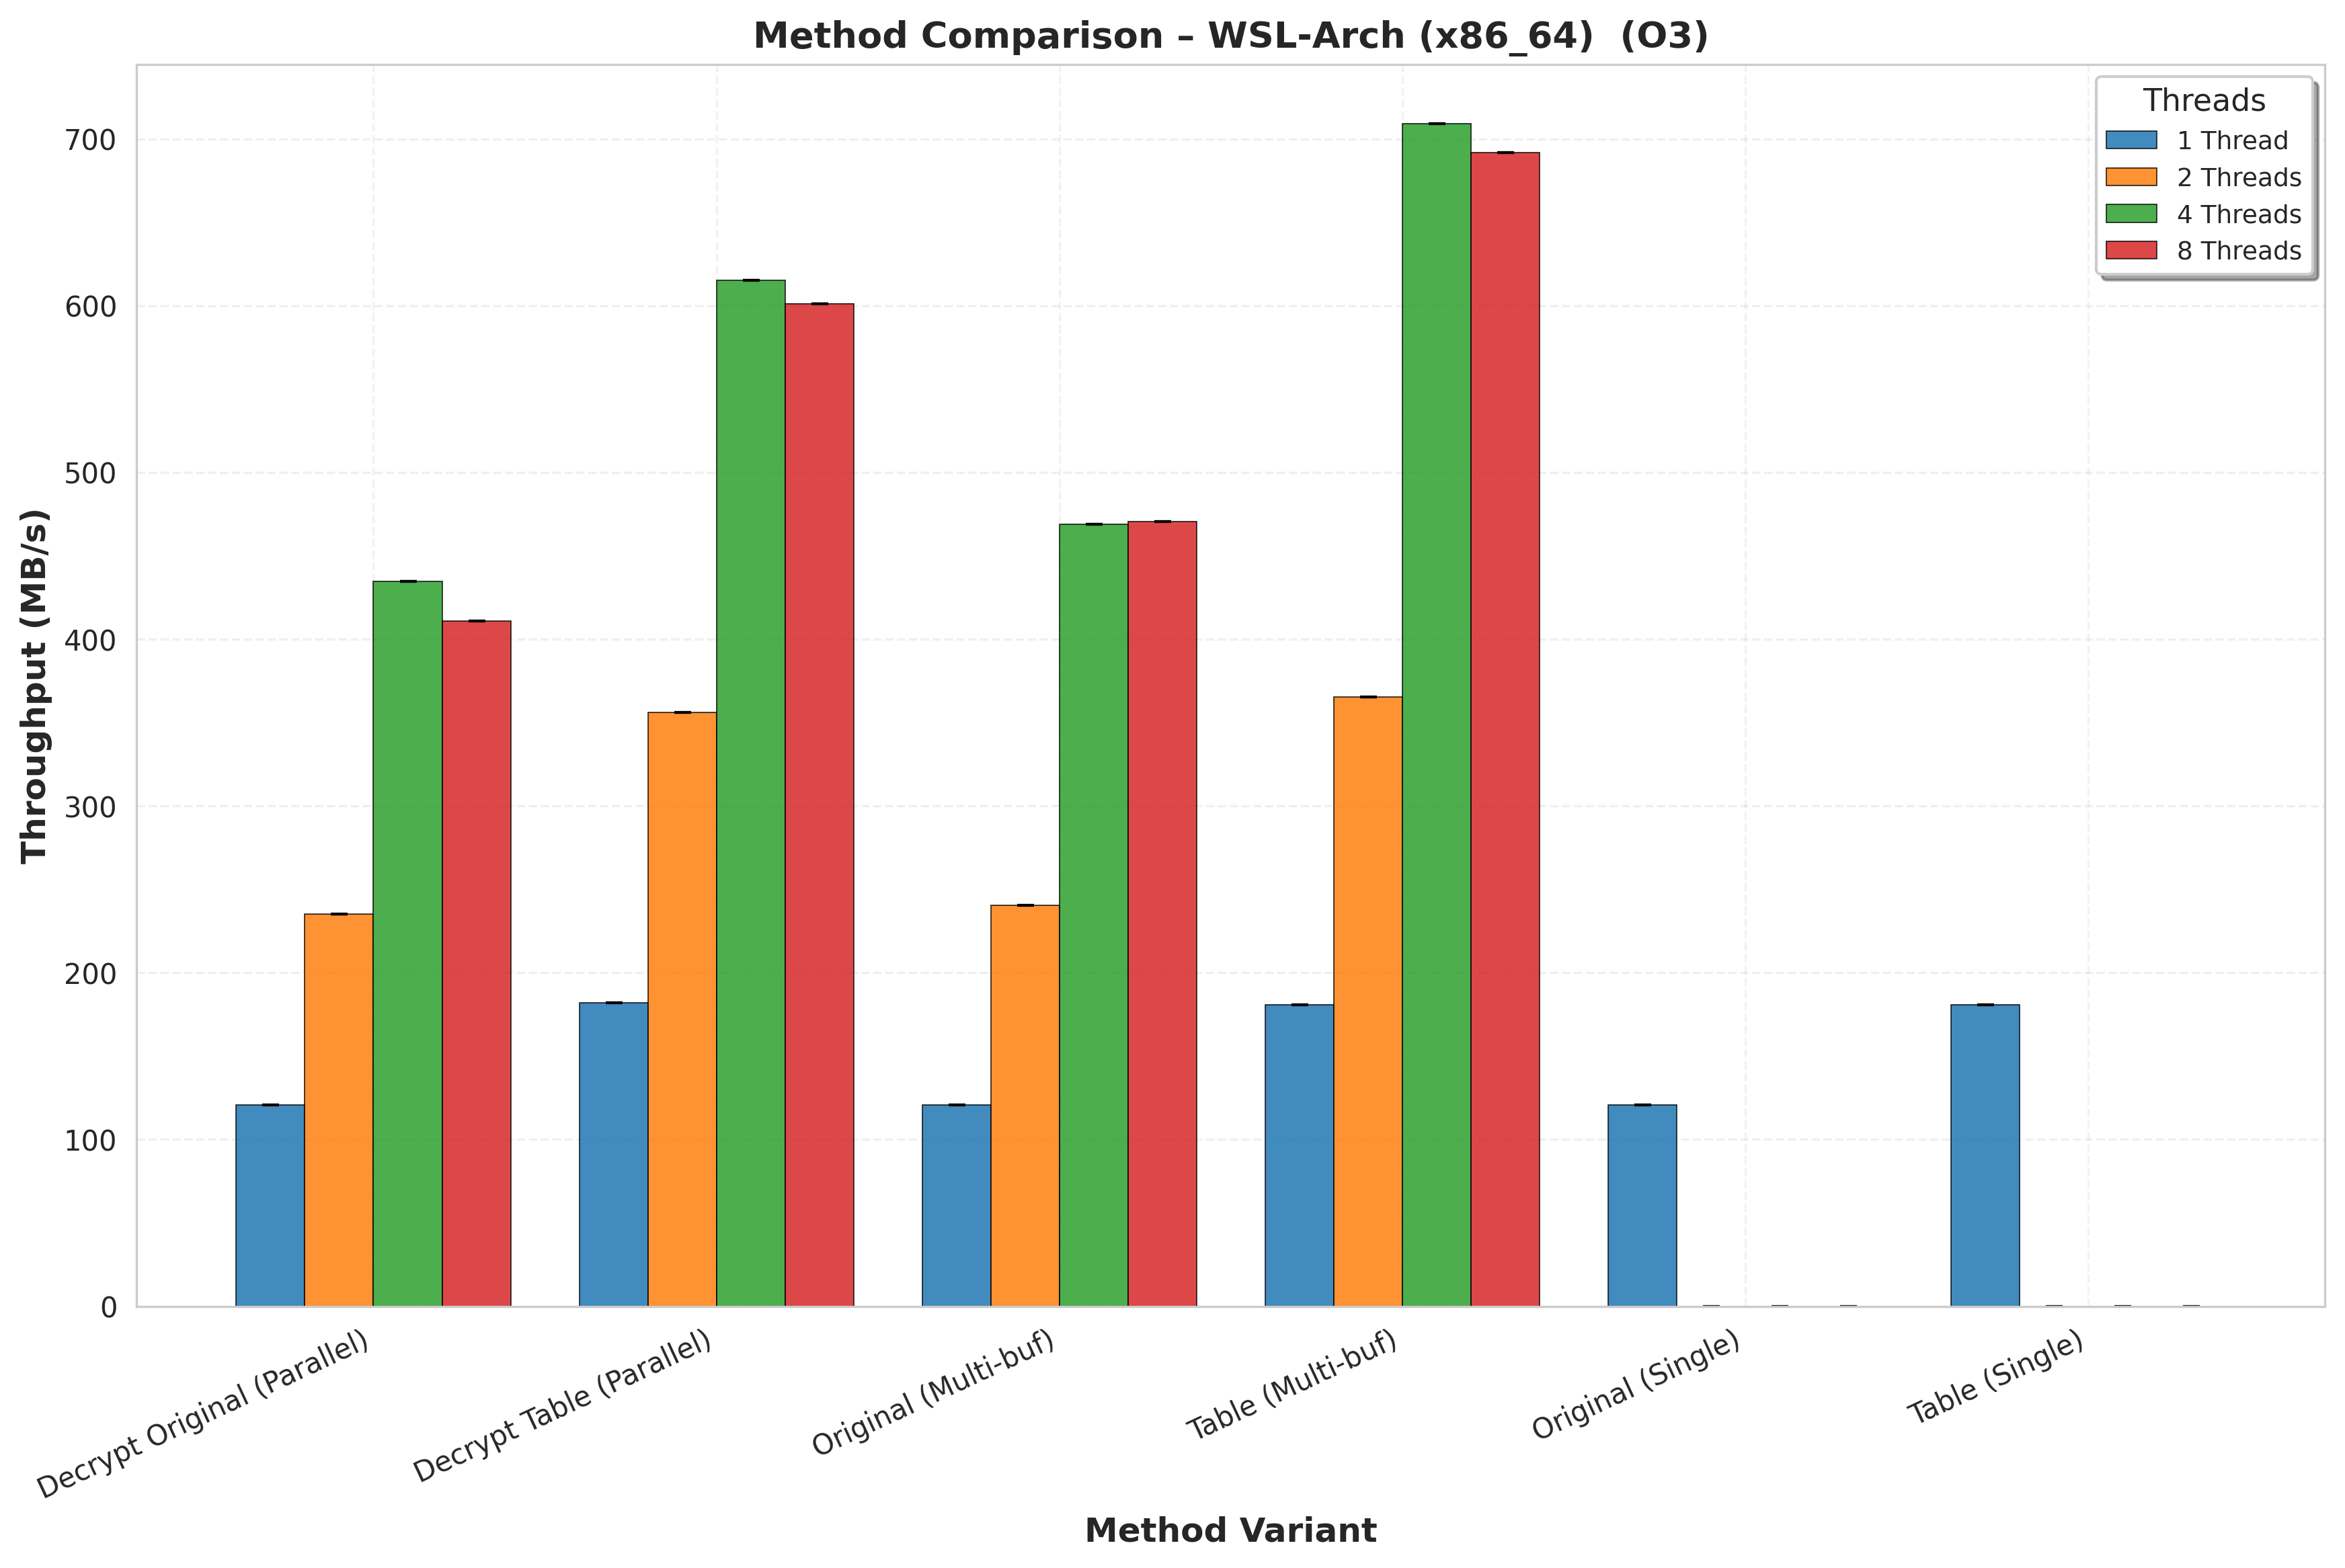
\includegraphics[width=\textwidth]{figure/bar_method_wsl-arch_O3_by_threads.png}
    \caption{WSL-Arch平台各变体吞吐量对比（O3）}
    \label{fig:method_wsl}
\end{figure}

\begin{figure}[H]
    \centering
    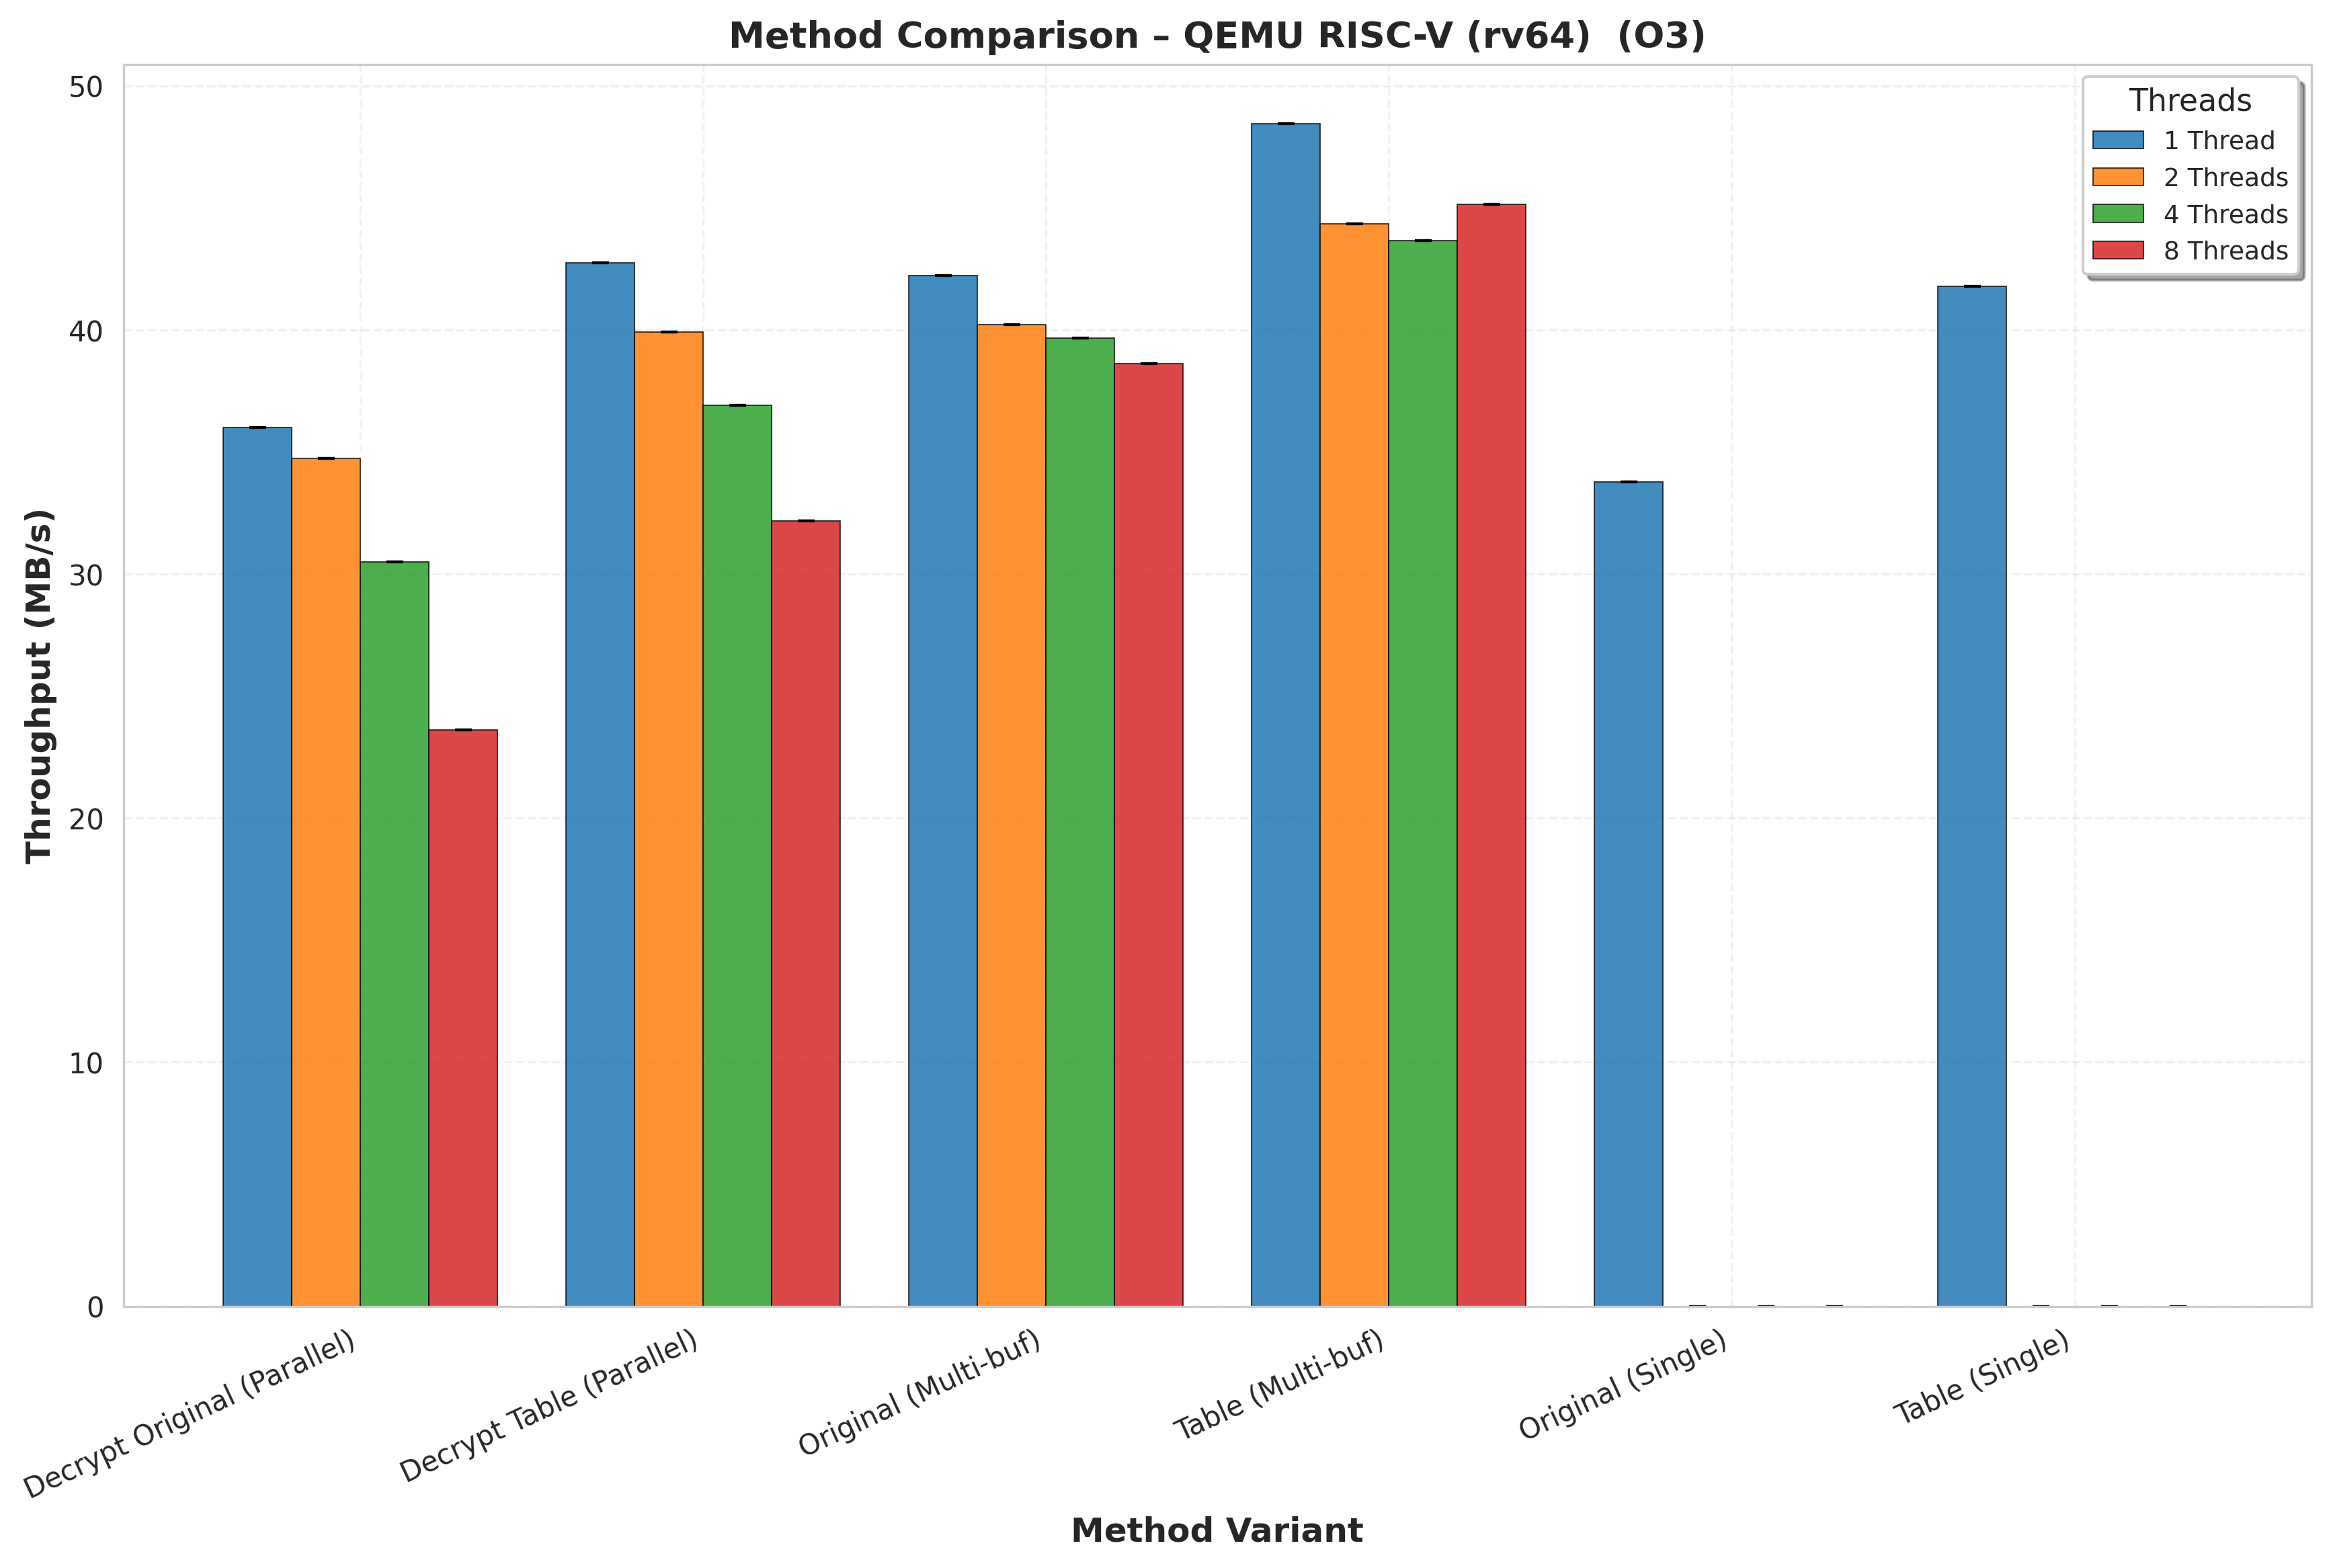
\includegraphics[width=\textwidth]{figure/bar_method_qemu-riscv_O3_by_threads.png}
    \caption{QEMU-RISC-V平台各变体吞吐量对比（O3）}
    \label{fig:method_qemu}
\end{figure}

分析要点：
\begin{enumerate}
    \item \textbf{查表优化效果显著}：在相同线程配置下，table变体的吞吐量普遍高于original变体。
          例如单线程O3下,WSL-Arch的single\_table达到180.83MB/s,相对single\_original的120.76MB/s提升约49.7\%；QEMU-RISC-V中single\_table达到41.79MB/s,相对single\_original的33.77MB/s提升约23.7\%。
    \item \textbf{多缓冲区并行加密}：multibuffer变体利用多缓冲区技术将多个独立加密任务并行处理，
          在WSL-Arch上多线程扩展性良好；但在QEMU-RISC-V上受限于仿真开销与单核性能，
          多线程带来的增益相对有限。
    \item \textbf{并行解密}：CBC模式的解密过程各密文分组之间无数据依赖，天然可并行化。
          decrypt\_parallel变体充分利用了这一特性，在多线程配置下获得显著的吞吐量提升。
    \item \textbf{线程扩展性}：WSL-Arch平台从1线程到4线程吞吐量提升明显,其中O3下multibuffer\_table在4线程达到709.34MB/s；
          QEMU-RISC-V平台在当前启动参数下多线程几乎没有带来收益,多数O3变体的最高吞吐量出现在1线程配置。
\end{enumerate}

\subsection{加密与解密性能对比}

图~\ref{fig:enc_vs_dec}展示了O3优化级别下加密（multi-buffer）与解密（parallel）的吞吐量
随线程数变化曲线。

\begin{figure}[H]
    \centering
    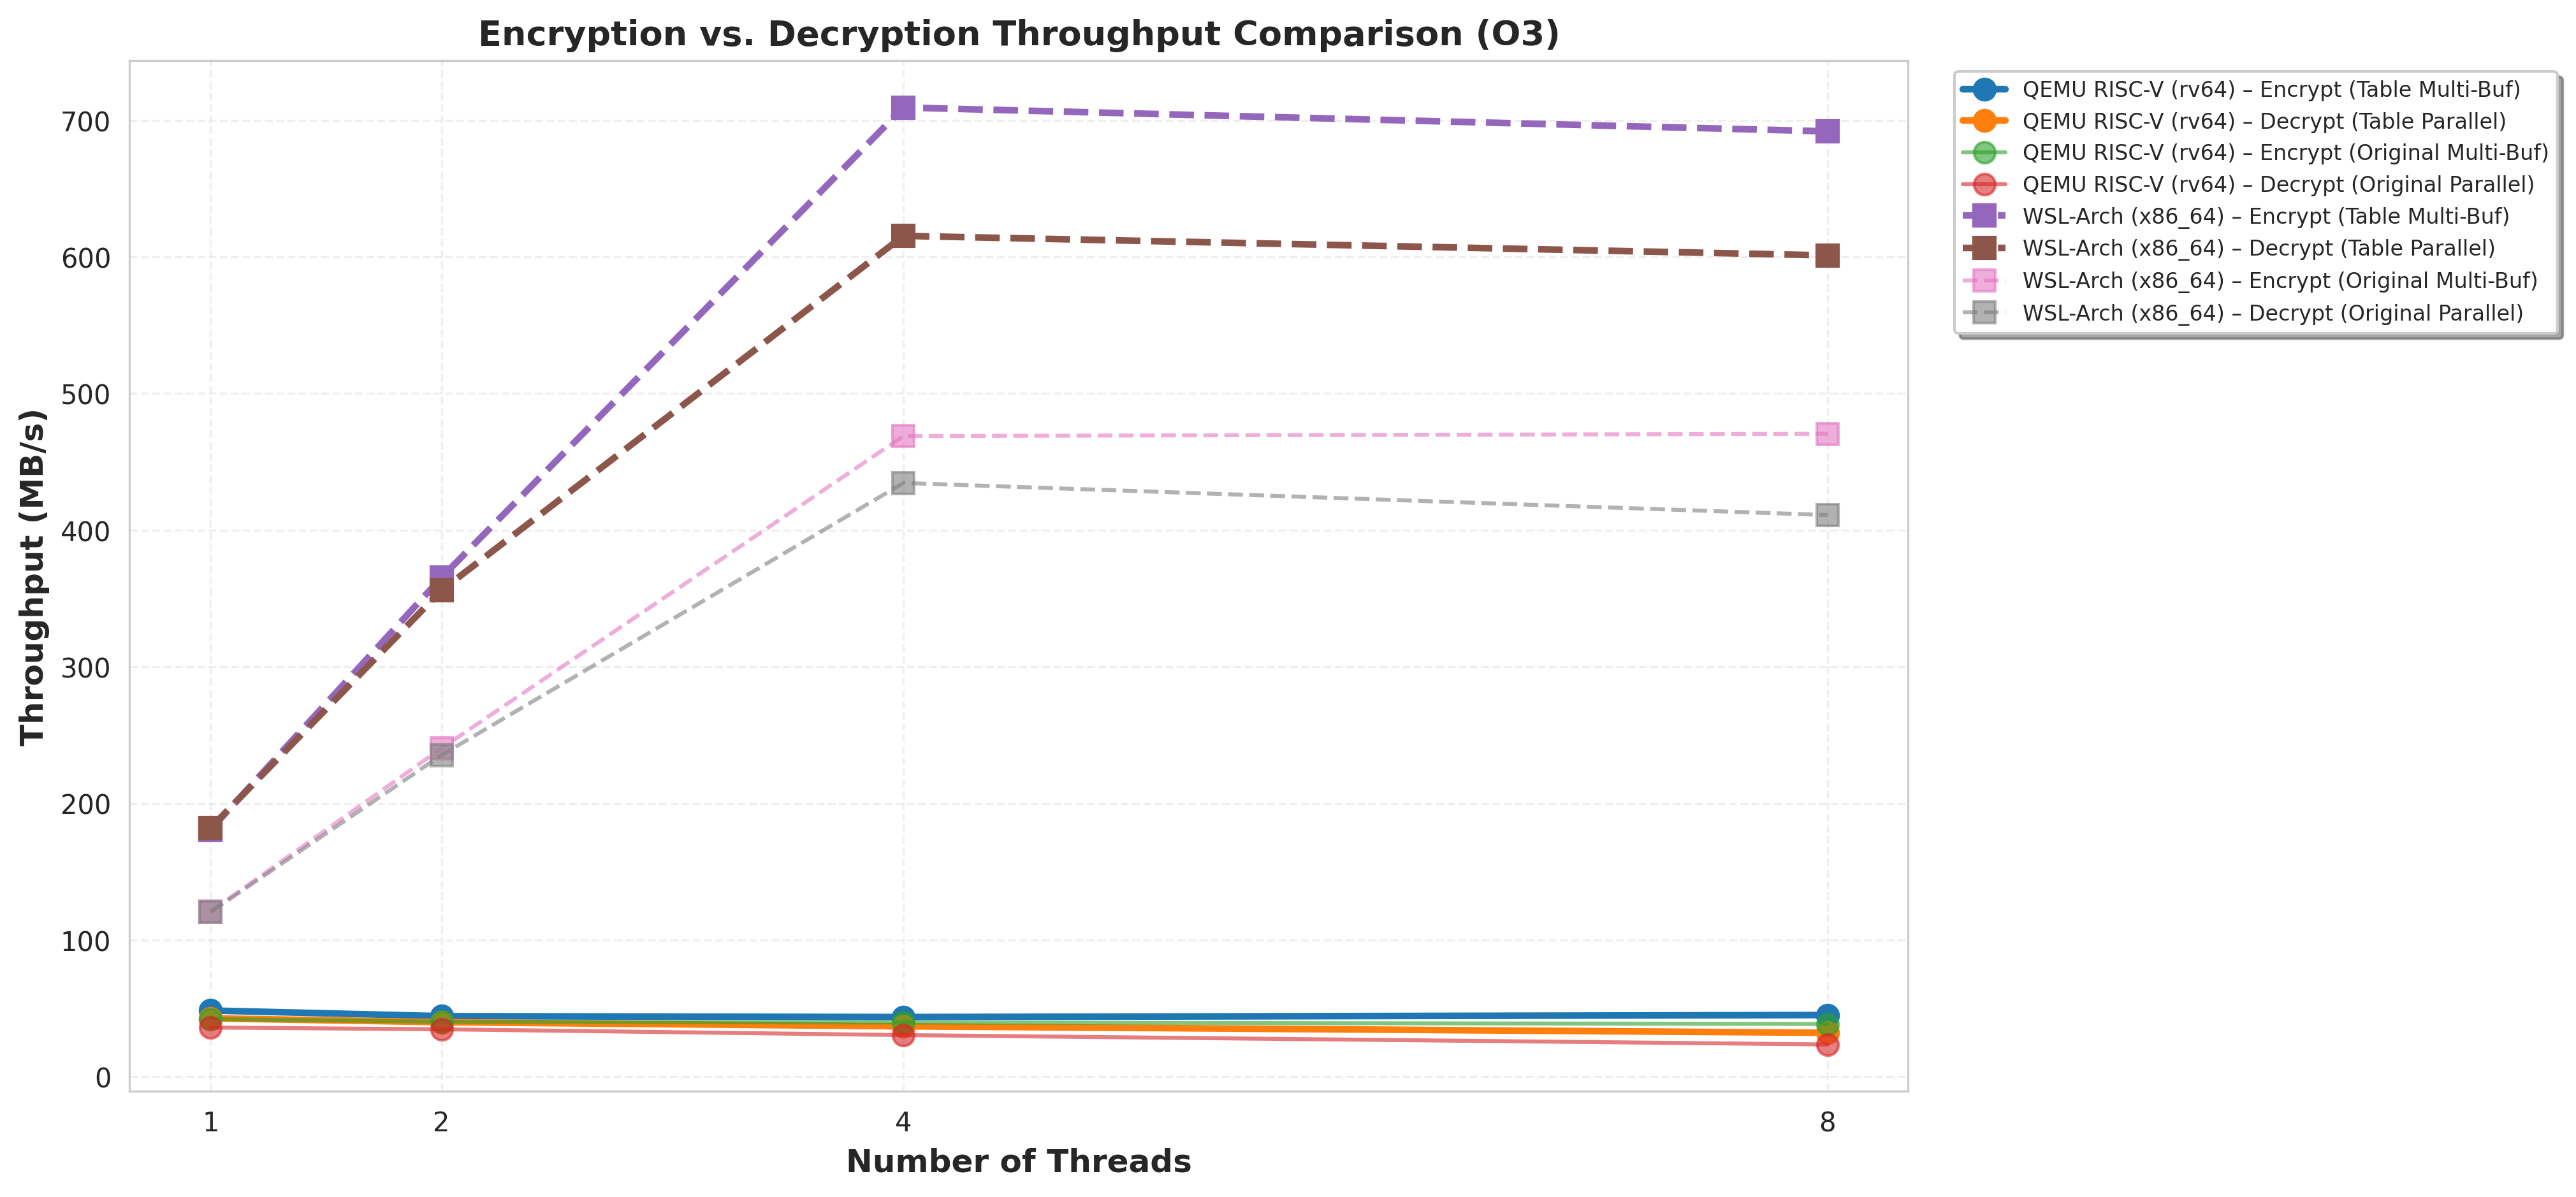
\includegraphics[width=\textwidth]{figure/line_encrypt_vs_decrypt_O3.png}
    \caption{加密vs解密吞吐量对比（O3）}
    \label{fig:enc_vs_dec}
\end{figure}

\textbf{关键发现}：
\begin{enumerate}
    \item CBC解密具备分组级并行条件,但实验结果还受到线程划分、线程创建开销和缓存竞争影响。在WSL-Arch的O3测试中,并行解密查表版本4线程达到615.41MB/s,明显高于其1线程的182.07MB/s。
    \item 多缓冲区加密并非单条CBC消息的分组并行,而是同时处理多条独立消息。该模式在WSL-Arch上同样取得较好扩展性,multibuffer\_table在4线程达到709.34MB/s。
    \item 在QEMU-RISC-V上,加密与解密的绝对吞吐量均较低,且多线程版本没有表现出主机环境中的扩展性。这说明当前QEMU配置更适合验证RISC-V功能正确性和单线程优化趋势,不适合作为真实多核RISC-V硬件的并行性能代表。
\end{enumerate}

\subsection{编译器优化级别的影响}

图~\ref{fig:opt_impact_wsl}与图~\ref{fig:opt_impact_qemu}展示了单线程条件下
各变体在不同编译器优化级别（O0-O3）下的吞吐量。

\begin{figure}[H]
    \centering
    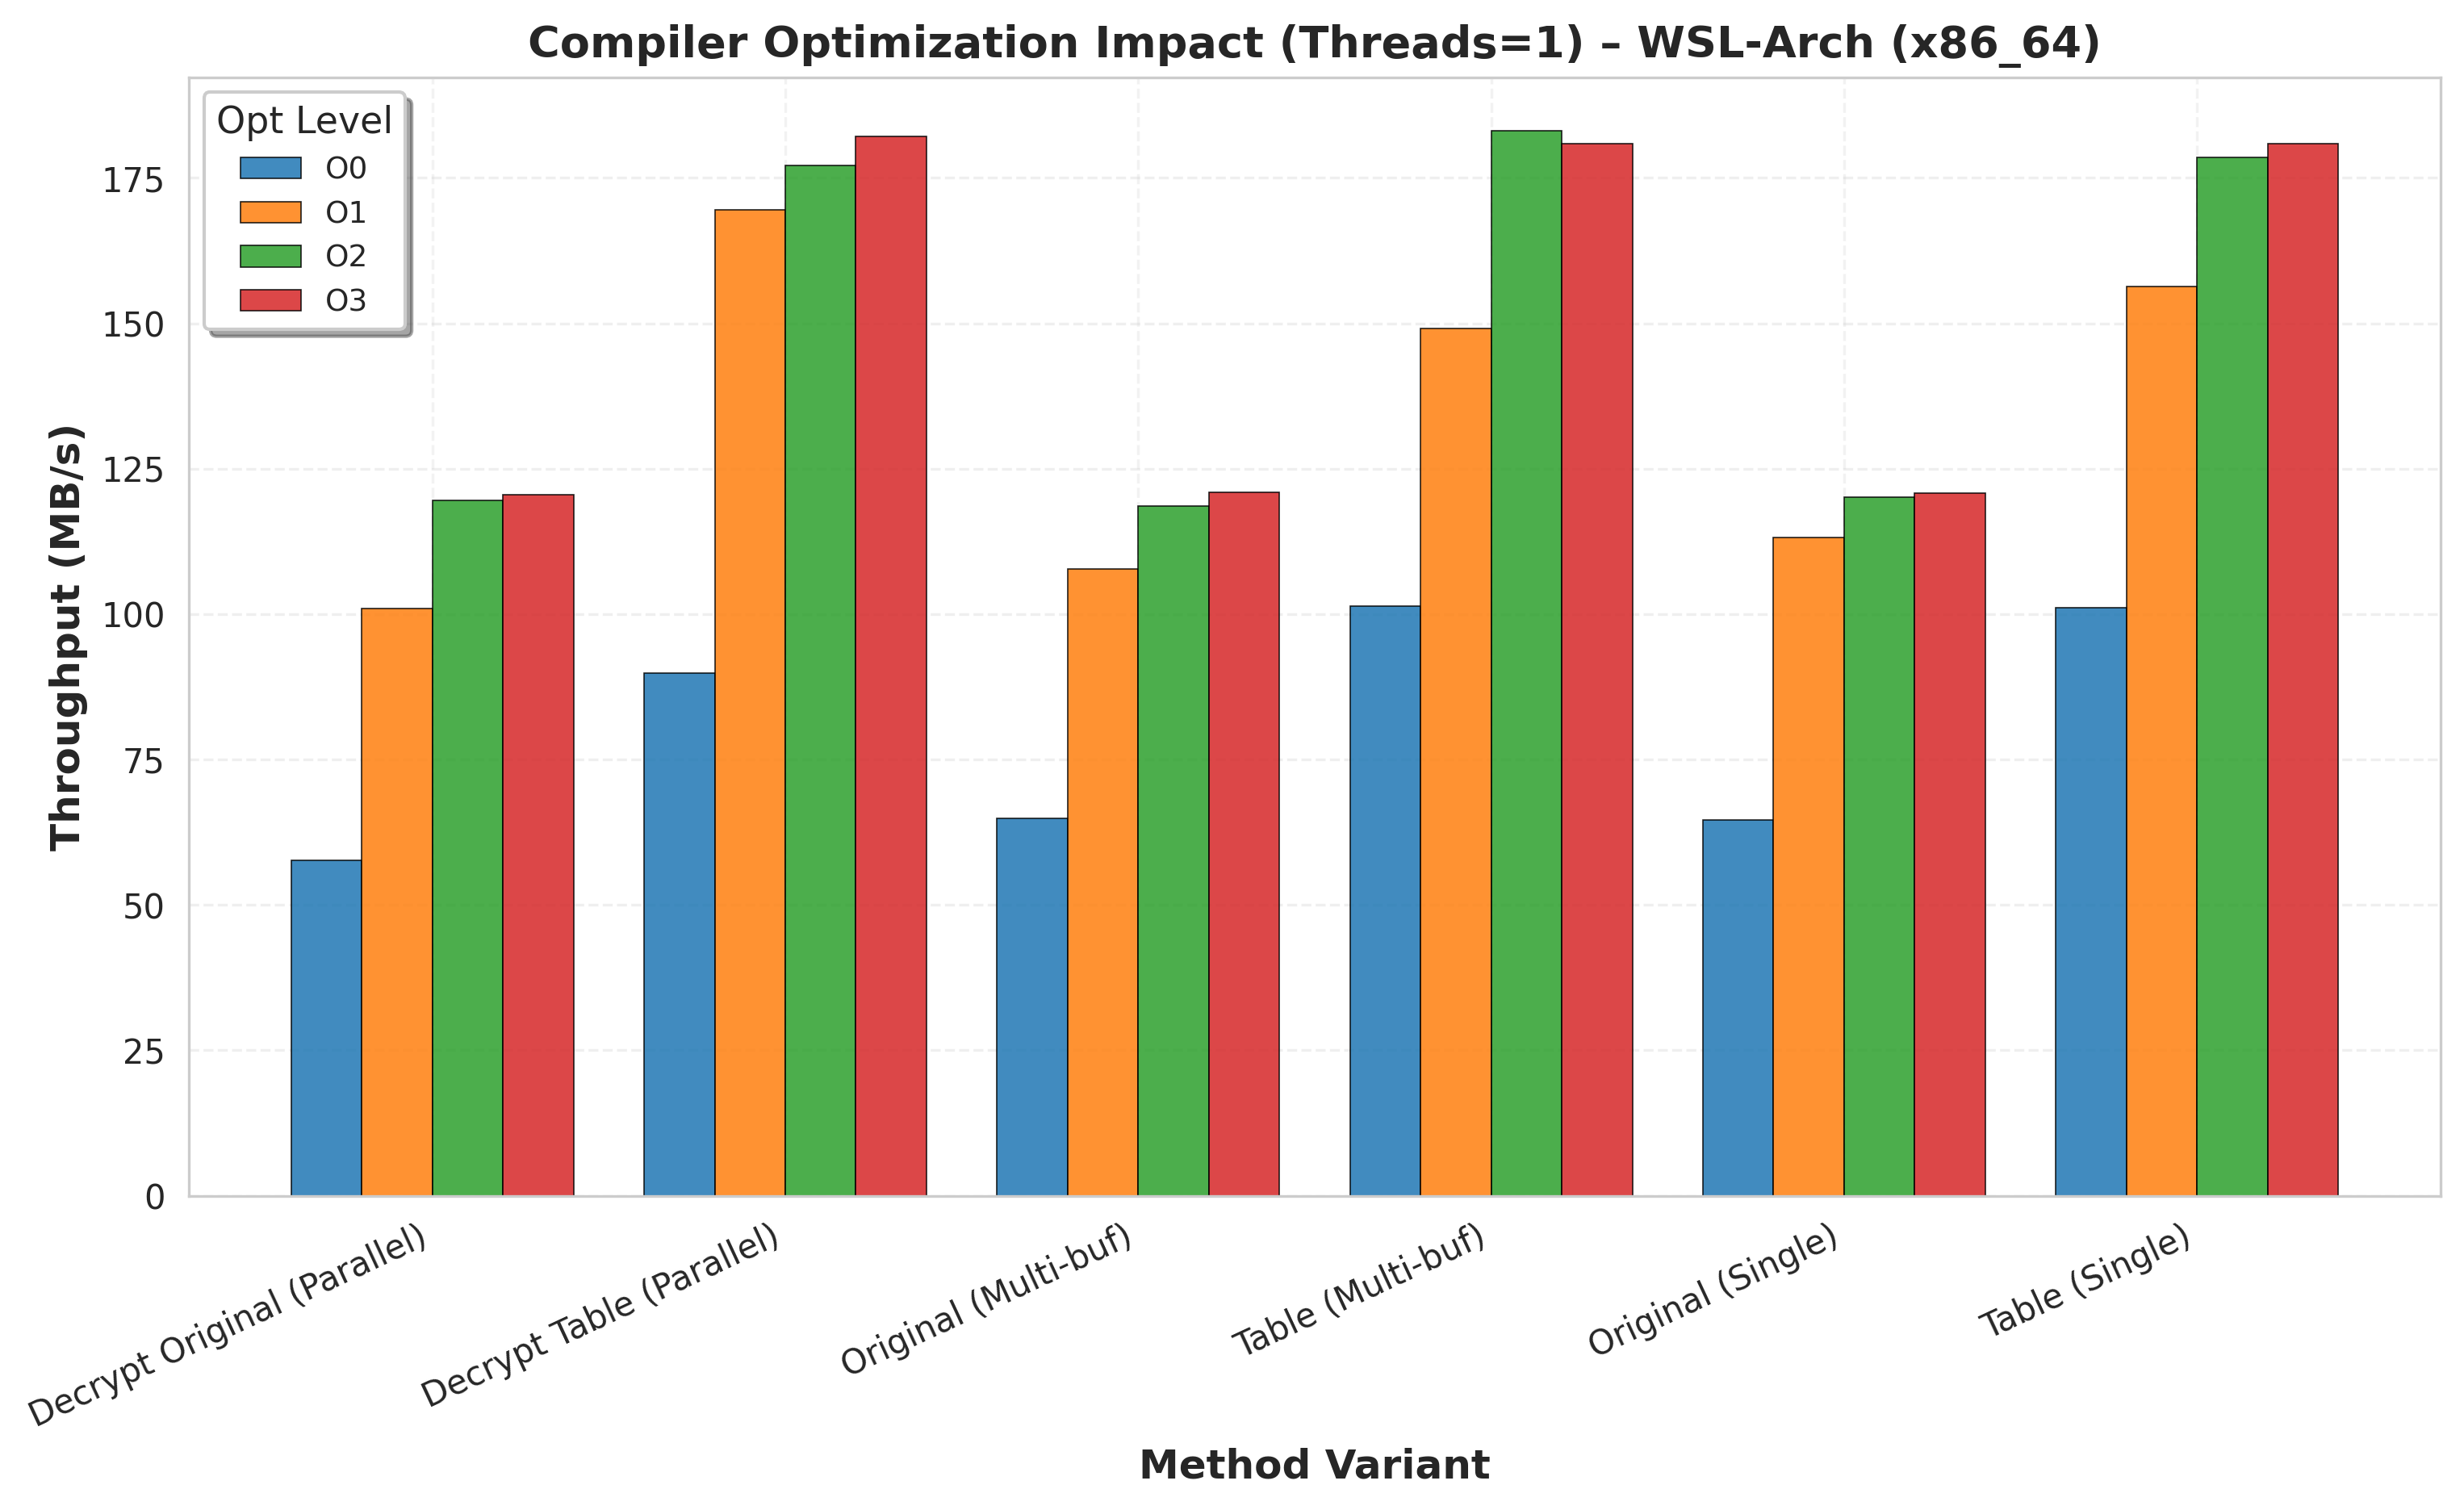
\includegraphics[width=\textwidth]{figure/bar_opt_impact_wsl-arch_t1.png}
    \caption{编译器优化影响 — WSL-Arch（单线程）}
    \label{fig:opt_impact_wsl}
\end{figure}

\begin{figure}[H]
    \centering
    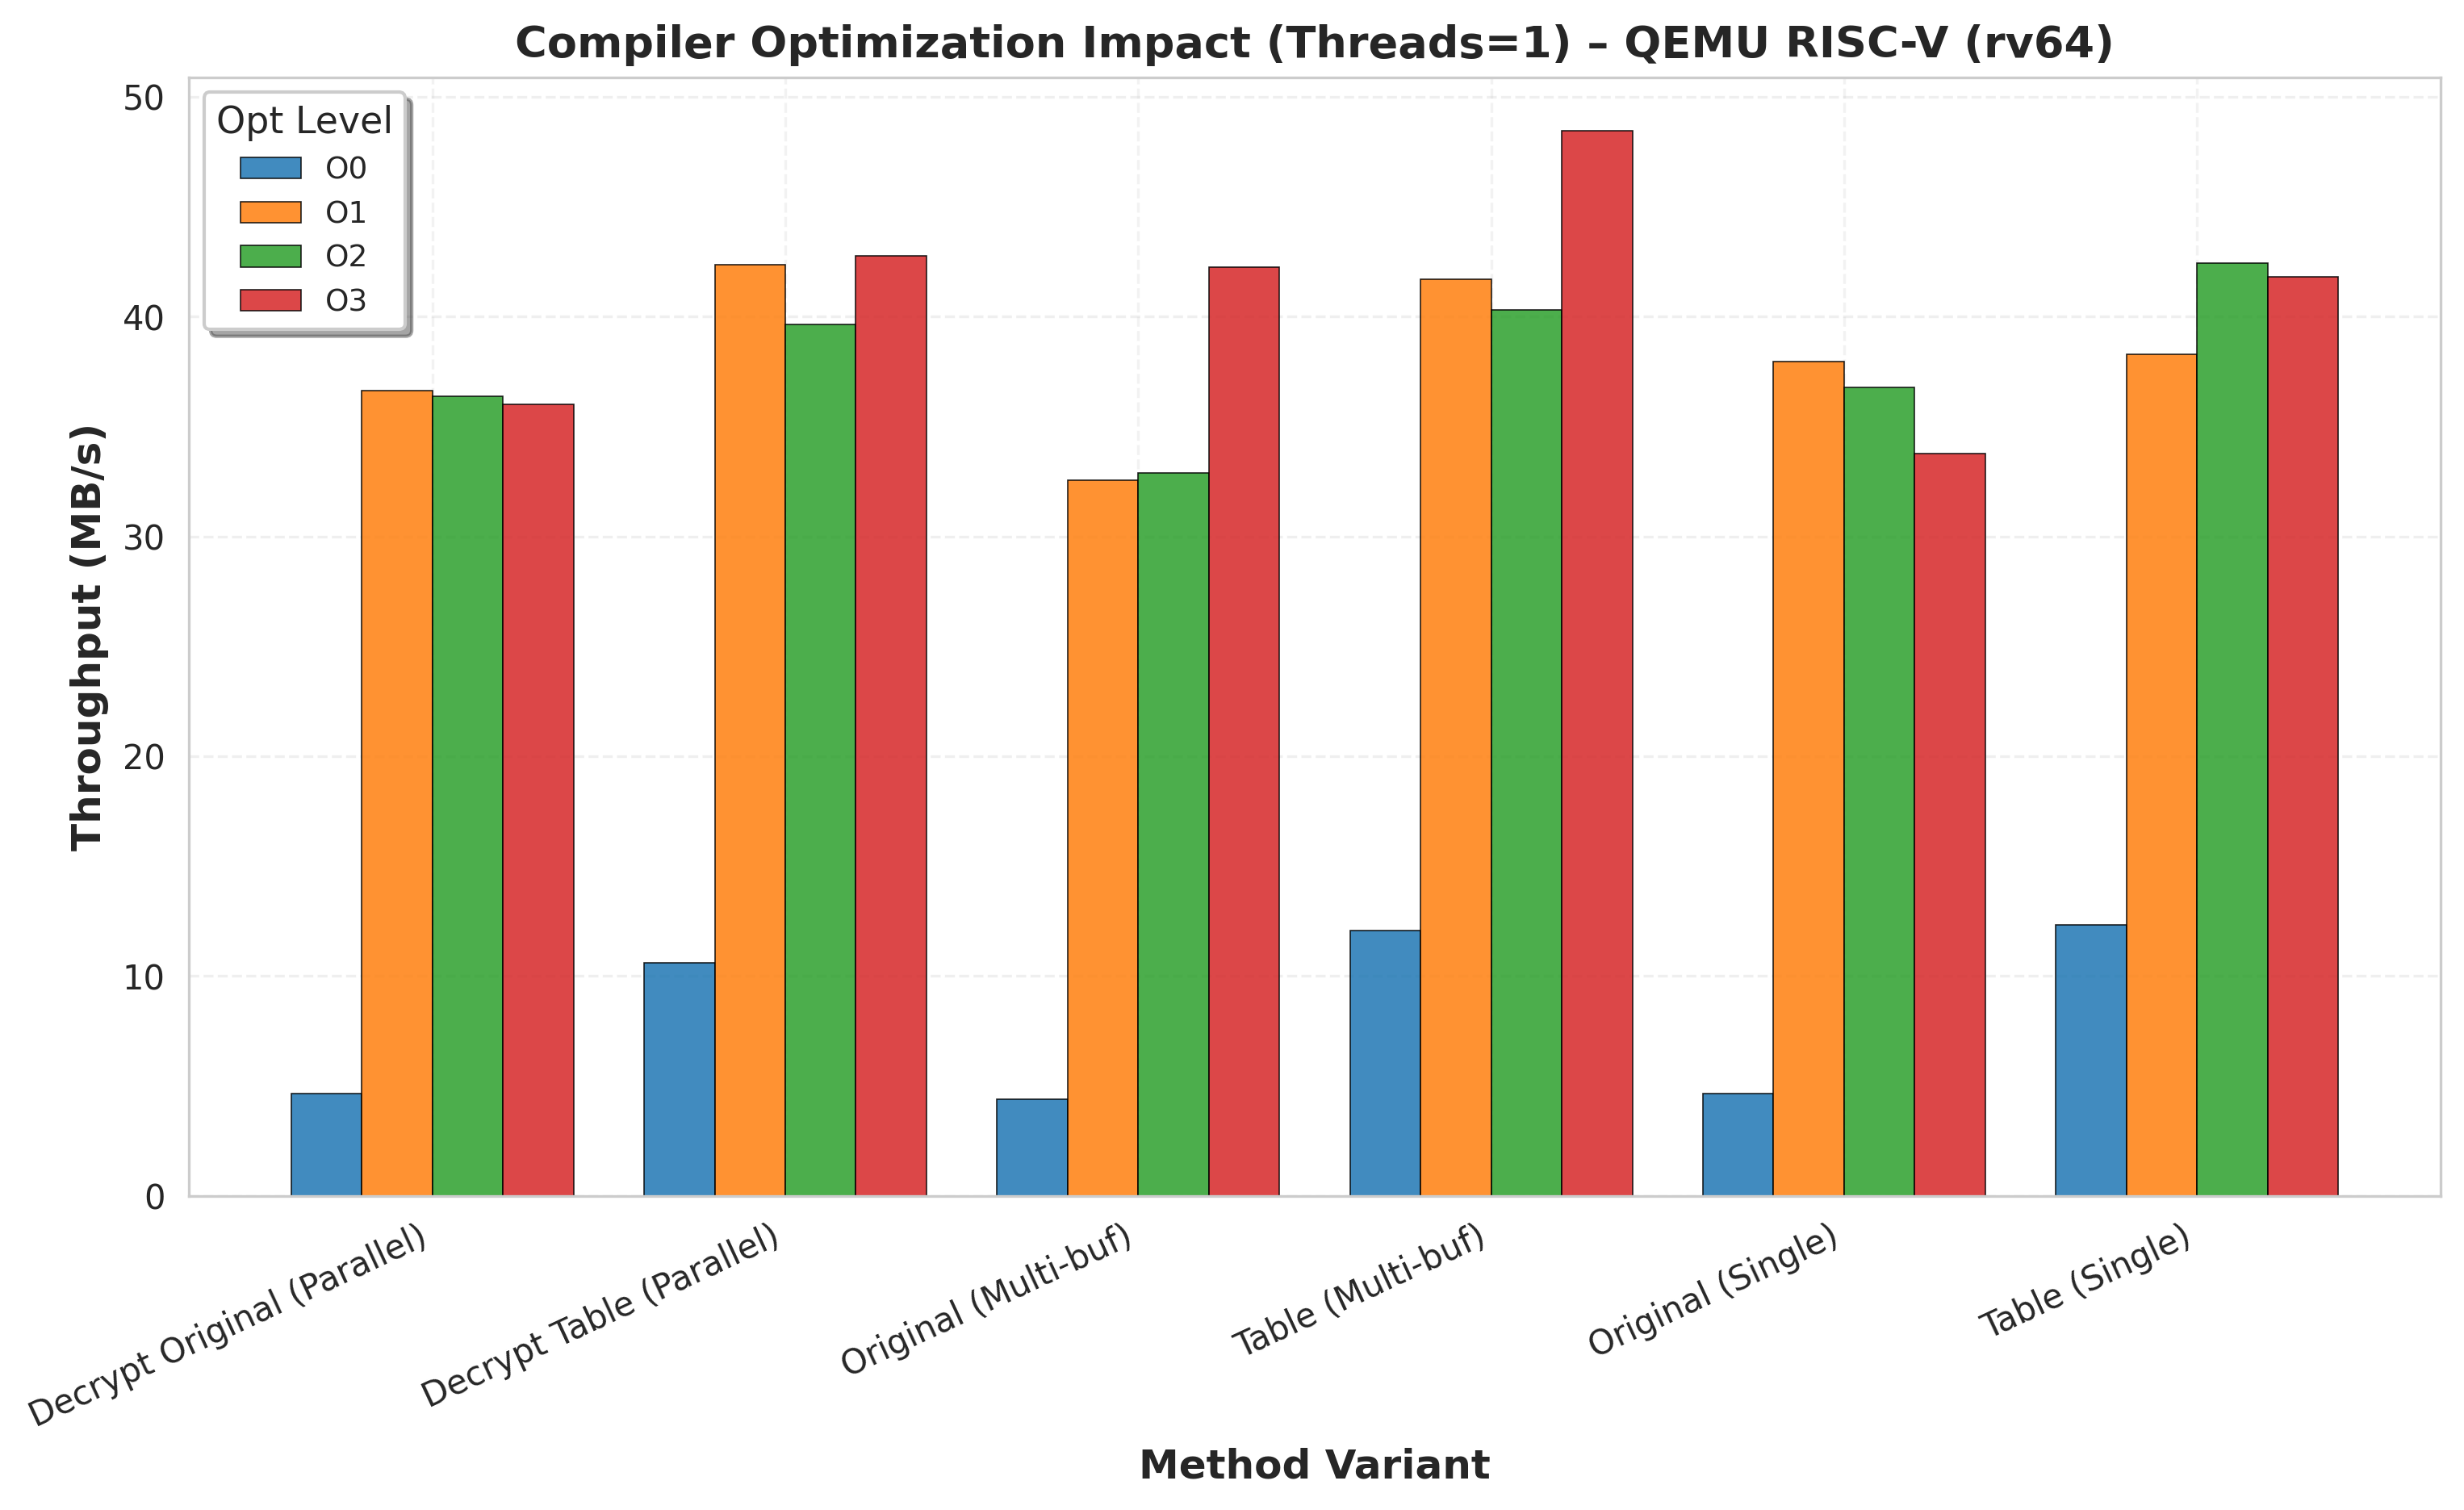
\includegraphics[width=\textwidth]{figure/bar_opt_impact_qemu-riscv_t1.png}
    \caption{编译器优化影响 — QEMU-RISC-V（单线程）}
    \label{fig:opt_impact_qemu}
\end{figure}

分析：
\begin{enumerate}
    \item WSL-Arch平台：原始版本从O0的64.60MB/s提升到O3的120.76MB/s,查表版本从O0的101.08MB/s提升到O3的180.83MB/s。编译器优化和查表优化可以叠加发挥作用。
    \item QEMU-RISC-V平台：原始版本从O0的4.65MB/s提升到O3的33.77MB/s,查表版本从O0的12.31MB/s提升到O3的41.79MB/s。O0代码在RISC-V模拟环境中开销很高,优化级别提升对循环、函数调用和寄存器使用的改善更加明显。
\end{enumerate}

\subsection{全维度总览}

图~\ref{fig:full_overview}以2×2子图形式汇总了四种优化级别下所有变体与平台的
吞吐量-线程数关系曲线，便于快速横向对比。

\begin{figure}[H]
    \centering
    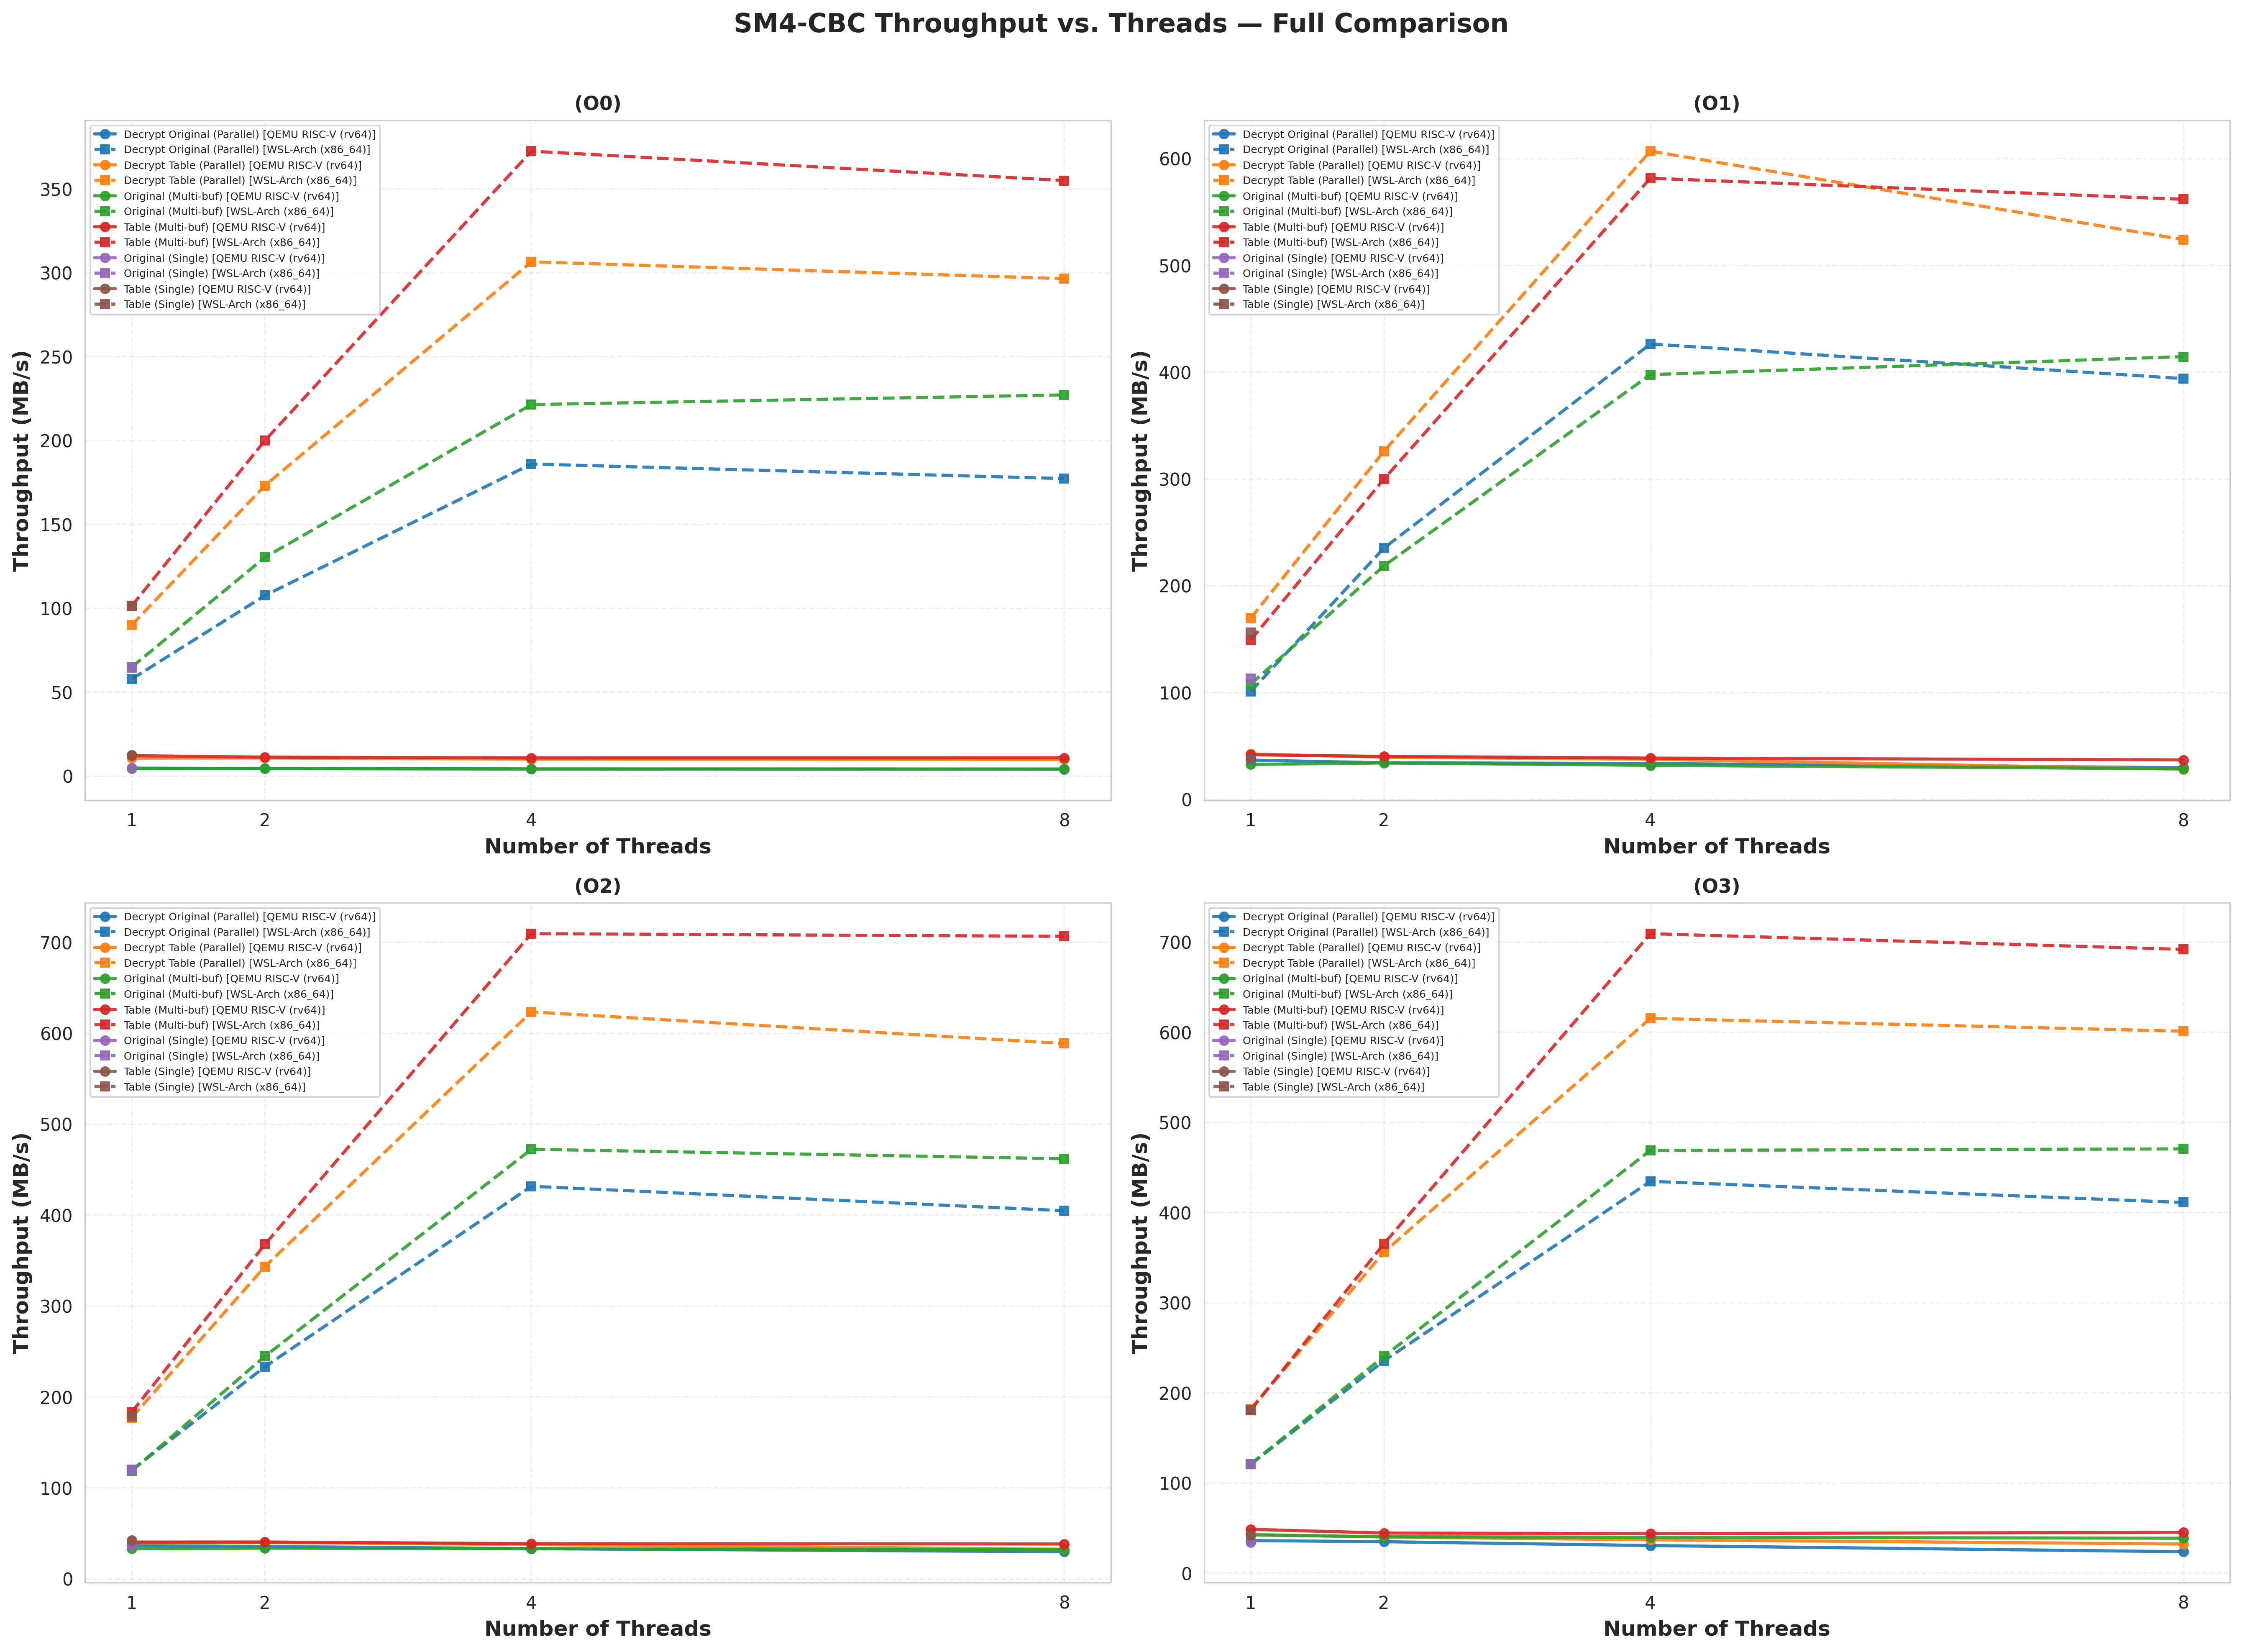
\includegraphics[width=\textwidth]{figure/line_throughput_vs_threads_full.png}
    \caption{SM4-CBC吞吐量 vs 线程数全维度对比}
    \label{fig:full_overview}
\end{figure}
